\apendice{Especificación de Requisitos}

\section{Introducción}
En este apéndice, se profundizará en los objetivos y requisitos que debe de cumplir el proyecto. A continuación se detallarán los siguientes aspectos:
\begin{itemize}
    \item \textbf{Objetivos generales:} se plasman los objetivos generales que se pretenden alcanzar con el proyecto.
    \item \textbf{Catálogo de requisitos:} se listan todos los requisitos que definen el comportamiento de la aplicación.
    \item \textbf{Especificación de requisitos:} se detallan los casos de uso para facilitar la comprensión de las interacciones del usuario con la aplicación.
\end{itemize}

\section{Objetivos generales}
En este proyecto, se han definido unos objetivos que marcan la trayectoria que se debe de seguir para el desarrollo de este:
\begin{itemize}
    \item Visualización de las actividades de Moodle en un diagrama de Gantt
    \item Creación de tareas personales asociadas a un curso del usuario
    \item Filtrado general de toda la aplicación
\end{itemize}

\section{Catálogo de requisitos}
En este apartado, se definirán todos los requisitos funcionales y no funcionales del proyecto.

\subsection{Requisitos funcionales}
\begin{itemize}
    \item \textbf{RF1. - Inicio de sesión:} el usuario tiene que poder acceder a la aplicación, mediante el correo y contraseña de su plataforma Moodle. Además, podrá habilitar una opción para guardar su correo. También, se debe de proporcionar una opción de recuperación de contraseña.
        \begin{itemize}
            \item \textbf{RF1.1. - Recuperación de contraseña:} la aplicación tiene que permitir al usuario recuperar su contraseña en caso de olvido.
            \item \textbf{RF1.2. - Guardar correo de inicio de sesión:} el usuario tiene que poder guardar el correo con el que realizar el inicio de sesión.
        \end{itemize}
    \item \textbf{RF2. - Conexión con plataforma Moodle:} el usuario tiene que poder conectarse a una plataforma Moodle. Además, la aplicación verificará que se trata de un servidor Moodle.
    \item \textbf{RF3. - Cierre de sesión:} el usuario tiene que poder cerrar sesión el aplicación.
    \item \textbf{RF4. - Acceso a todas las funcionalidades desde la pantalla principal:} el usuario tiene que poder acceder a todas las funcionalidades de la aplicación desde la pantalla principal.
    \item \textbf{RF5. - Visualización de actividades en el diagrama de Gantt:} el usuario tiene que poder visualizar todas sus actividades (filtradas o sin filtrar) en el diagrama de Gantt. También, tendrá que poder ver una información mínima de cada actividad, así como modificar la estética del diagrama con filtros.
        \begin{itemize}
            \item \textbf{RF5.1. - Ver información de la actividad:} la aplicación tiene que permitir al usuario ver una previsualización de la actividad desde el propio diagrama.
            \item \textbf{RF5.2. - Cambiar estética del diagrama:} la aplicación tiene que permitir al usuario modificar la estética del diagrama de Gantt. 
        \end{itemize}
    \item \textbf{RF6. - Visualización de actividades en la sección de actividades del diagrama:} el usuario tiene que poder ver las mismas actividades del diagrama en el sección de actividades, pero con más información que pueda resultar relevante.
        \begin{itemize}
            \item \textbf{RF6.1. - Visualizar tarjeta de la actividad:} la aplicación tiene que permitir al usuario visualizar toda la información disponible de la actividad.
        \end{itemize}
    \item \textbf{RF7. - Visualización de tareas personales:} el usuario tiene que poder ver todas sus tareas personales repartidas en las dos secciones disponibles, así como la información de cada tarea.
        \begin{itemize}
            \item \textbf{RF7.1. - Visualizar información de tarea personal:} la aplicación tiene que permitir al usuario visualizar toda la información de la tarea personal.
            \item \textbf{RF7.2. - Marcar realización de tarea personal:} la aplicación tiene que permitir al usuario cambiar el estado de finalización de la tarea personal.
            \item \textbf{RF7.3. - Borrar tarea personal:} la aplicación tiene que permitir al usuario eliminar la tarea personal.
        \end{itemize}
    \item \textbf{RF8. - Creación de tareas personales:} el usuario tiene que poder crear sus propias tareas personales.
    \item \textbf{RF9. - Filtrar contenidos de la aplicación:} el usuario tiene que poder filtrar todos los contenidos de la aplicación, tanto actividades de Moodle como tareas personales.
\end{itemize}

\subsection{Requisitos no funcionales}
\begin{itemize}
    \item \textbf{RNF1. - Disponibilidad:} la aplicación debe de garantizar su completa disponibilidad, independientemente de la ubicación del usuario.
    \item \textbf{RNF2. - Usabilidad:} la aplicación debe de garantizar al usuario un uso sencillo e intuitivo.
    \item \textbf{RNF3. - Mantenimiento:} la aplicación debe de aportar facilidad en el mantenimiento para la corrección de errores.
    \item \textbf{RNF4. - Escalabilidad:} la aplicación debe de ser capaz de gestionar un crecimiento de usuarios sin afectar negativamente a su rendimiento.
    \item \textbf{RNF5. - Rendimiento:} la aplicación debe de tener tiempos de respuesta y cargas de datos aceptables, para que la experiencia de usuario sea fluida.
    \item \textbf{RNF6. - Seguridad:} la aplicación debe de garantizar la protección de los datos del usuario.
\end{itemize}

\section{Especificación de requisitos}

\subsection{Actores del sistema}
\begin{table}[H]
	\centering
	\begin{tabularx}{\linewidth}{ p{0.21\columnwidth} p{0.71\columnwidth} }
		\toprule
		\textbf{Actor}    & \textbf{A01}\\
		\toprule
            \textbf{Nombre}              & Usuario    \\
		\textbf{Versión}              & 1.0    \\
		\textbf{Autor}                & Javier Pampliega García \\
		\textbf{Descripción}          & Persona que hace uso de la aplicación para planificar sus actividades Moodle y tareas personales. \\
		\textbf{Tipo}         & Usuario \\
            \textbf{Objetivo}         & Visualizar y planificar actividades Moodle, y crear y gestionar tareas personales.\\
		\textbf{Responsabilidades}             &
		\begin{itemize}
			\def\labelenumi{\arabic{enumi}.}
			\tightlist
                \item Iniciar sesión para conectarse a Moodle.
			\item Usar el sistema de filtrado.
			\item Visualizar diagrama de Gantt y actividades.
                \item Crear y gestionar tareas personales.
		\end{itemize}\\
		\textbf{Relaciones con casos de uso}        &  \\
		\bottomrule
	\end{tabularx}
	\caption{A01 - Usuario}
\end{table}

\begin{table}[H]
	\centering
	\begin{tabularx}{\linewidth}{ p{0.21\columnwidth} p{0.71\columnwidth} }
		\toprule
		\textbf{Actor}    & \textbf{A02}\\
		\toprule
            \textbf{Nombre}              & API de Moodle    \\
		\textbf{Versión}              & 1.0    \\
		\textbf{Autor}                & Javier Pampliega García \\
		\textbf{Descripción}          &  \\
		\textbf{Tipo}         & Sistema \\
            \textbf{Objetivo}         & Obtener todos los datos necesarios para el funcionamiento de la aplicación.\\
		\textbf{Responsabilidades}             &
		\begin{itemize}
			\def\labelenumi{\arabic{enumi}.}
			\tightlist
                \item Obtención de los datos de Moodle del usuario del usuario.
		\end{itemize}\\
		\textbf{Relaciones con casos de uso}        &  \\
		\bottomrule
	\end{tabularx}
	\caption{A02 - API de Moodle}
\end{table}

\begin{table}[H]
	\centering
	\begin{tabularx}{\linewidth}{ p{0.21\columnwidth} p{0.71\columnwidth} }
		\toprule
		\textbf{Actor}    & \textbf{A03}\\
		\toprule
            \textbf{Nombre}              & Supabase    \\
		\textbf{Versión}              & 1.0    \\
		\textbf{Autor}                & Javier Pampliega García \\
		\textbf{Descripción}          & Servicio en la nube que posibilita el almacenamiento de datos en la nube. \\
		\textbf{Tipo}         & Sistema \\
            \textbf{Objetivo}         & Insertar y borrar tareas personales del usuario en la nube.\\
		\textbf{Responsabilidades}             &
		\begin{itemize}
			\def\labelenumi{\arabic{enumi}.}
			\tightlist
                \item Almacenar las tareas creadas del usuario.
			\item Cargar las tareas del usuario.
			\item Eliminar del almacenamiento en la nube las tareas del usuario.
		\end{itemize}\\
		\textbf{Relaciones con casos de uso}        &  \\
		\bottomrule
	\end{tabularx}
	\caption{A03 - Supabase}
\end{table}

\subsection{Casos de uso}
\begin{figure}[t]
    \centering
    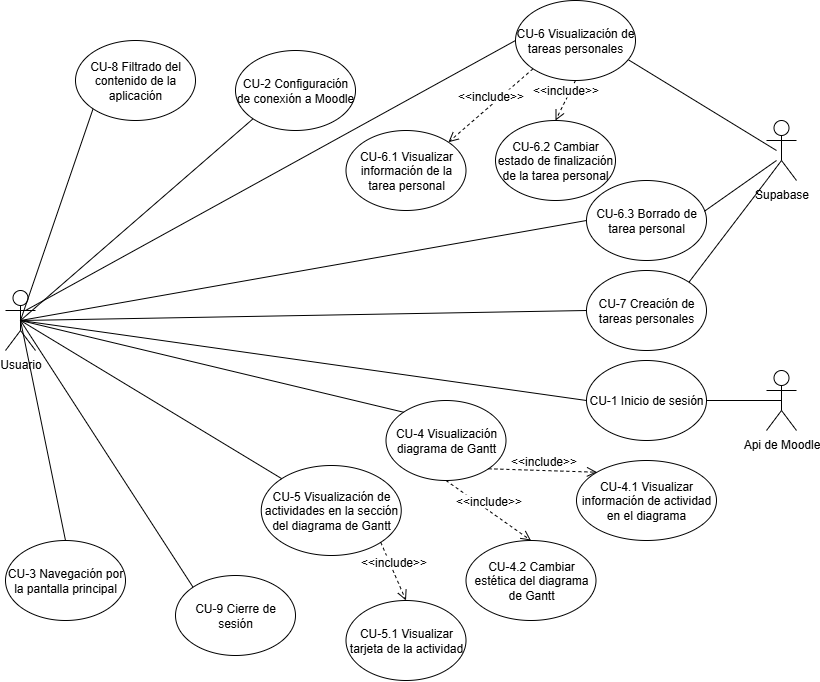
\includegraphics[width=1.0\linewidth]{img/diagrama_casos_uso.png}
    \caption{Diagrama general de los casos de uso}
    \label{fig:diagrama_casos_uso}
\end{figure}

\begin{table}[H]
	\centering
	\begin{tabularx}{\linewidth}{ p{0.21\columnwidth} p{0.71\columnwidth} }
		\toprule
		\textbf{CU-1}    & \textbf{Inicio de sesión}\\
		\toprule
		\textbf{Versión}              & 1.0    \\
            \textbf{Actor}                & Usuario, API de Moodle \\
		\textbf{Autor}                & Javier Pampliega García \\
		\textbf{Requisitos asociados} & RF-1\\
		\textbf{Descripción}          & Permitir iniciar sesión para acceder a la aplicación y para cargar los datos de Moodle. \\
		\textbf{Precondición}         & La aplicación instalada y abierta. \\
		\textbf{Acciones}             &
		\begin{enumerate}
			\def\labelenumi{\arabic{enumi}.}
			\tightlist
			\item Estar conectado a una plataforma Moodle.
			\item Introducir las credenciales de usuario.
                \item Presionar el botón de inicio de sesión.
		\end{enumerate}\\
		\textbf{Postcondición}        & Inicio de sesión con la cuenta de Moodle del usuario. \\
		\textbf{Excepciones}          & \begin{itemize}
		    \item Ausencia de plataforma Moodle configurada.
                \item Credenciales incorrectas.
                \item Ausencia de conexión a Internet.
		\end{itemize} \\
		\textbf{Importancia}          & Alta \\
		\bottomrule
	\end{tabularx}
	\caption{CU-1 Inicio de sesión}
\end{table}

\begin{table}[p]
	\centering
	\begin{tabularx}{\linewidth}{ p{0.21\columnwidth} p{0.71\columnwidth} }
		\toprule
		\textbf{CU-2}    & \textbf{Configuración de conexión a Moodle}\\
		\toprule
		\textbf{Versión}              & 1.0    \\
            \textbf{Actor}                & Usuario \\
		\textbf{Autor}                & Javier Pampliega García \\
		\textbf{Requisitos asociados} & RF-2\\
		\textbf{Descripción}          & Permitir conectar con un servidor de Moodle. \\
		\textbf{Precondición}         & La aplicación instalada y abierta, y en el panel para conectar con un servidor Moodle. \\
		\textbf{Acciones}             &
		\begin{enumerate}
			\def\labelenumi{\arabic{enumi}.}
			\tightlist
			\item Introducir la URL del servidor Moodle.
                \item Esperar la verificación de la URL.
			\item Presionar el botón Guardar.
		\end{enumerate}\\
		\textbf{Postcondición}        & Inicio de sesión con la cuenta de Moodle del usuario. \\
		\textbf{Excepciones}          & \begin{itemize}
		    \item Que no se trate de un servidor Moodle.
                \item Ausencia de conexión a Internet.
		\end{itemize} \\
		\textbf{Importancia}          & Alta \\
		\bottomrule
	\end{tabularx}
	\caption{CU-2 Configuración de conexión a Moodle}
\end{table}

\begin{table}[p]
	\centering
	\begin{tabularx}{\linewidth}{ p{0.21\columnwidth} p{0.71\columnwidth} }
		\toprule
		\textbf{CU-3}    & \textbf{Navegación por la pantalla principal}\\
		\toprule
		\textbf{Versión}              & 1.0    \\
            \textbf{Actor}                & Usuario \\
		\textbf{Autor}                & Javier Pampliega García \\
		\textbf{Requisitos asociados} & RF-4\\
		\textbf{Descripción}          & Permitir acceder a todas las funcionalidades de la aplicación desde la misma pantalla. \\
		\textbf{Precondición}         & Sesión iniciada correctamente. \\
		\textbf{Acciones}             &
		\begin{enumerate}
			\def\labelenumi{\arabic{enumi}.}
			\tightlist
			\item Pulsar el botón de la funcionalidad a la que se quiera acceder.
		\end{enumerate}\\
		\textbf{Postcondición}        & Acceso a la funcionalidad seleccionada. \\
		\textbf{Excepciones}          & \begin{itemize}
		    \item No existen excepciones.
		\end{itemize} \\
		\textbf{Importancia}          & Media \\
		\bottomrule
	\end{tabularx}
	\caption{CU-3 Navegación por la pantalla principal}
\end{table}

\begin{table}[p]
	\centering
	\begin{tabularx}{\linewidth}{ p{0.21\columnwidth} p{0.71\columnwidth} }
		\toprule
		\textbf{CU-4}    & \textbf{Visualización del diagrama de Gantt}\\
		\toprule
		\textbf{Versión}              & 1.0    \\
            \textbf{Actor}                & Usuario \\
		\textbf{Autor}                & Javier Pampliega García \\
		\textbf{Requisitos asociados} & RF-5\\
		\textbf{Descripción}          & Permitir visualizar todas las actividades (filtradas o sin filtrar) en un diagrama de Gantt. \\
		\textbf{Precondición}         & Haber accedido desde la pantalla principal. \\
		\textbf{Acciones}             &
		\begin{enumerate}
			\def\labelenumi{\arabic{enumi}.}
			\tightlist
			\item Desplazarse por el diagrama para ver todas las actividades.
		\end{enumerate}\\
		\textbf{Postcondición}        & No hay postcondiciones. \\
		\textbf{Excepciones}          & \begin{itemize}
		    \item No existen excepciones.
		\end{itemize} \\
		\textbf{Importancia}          & Alta \\
		\bottomrule
	\end{tabularx}
	\caption{CU-4 Visualización del diagrama de Gantt}
\end{table}

\begin{table}[p]
	\centering
	\begin{tabularx}{\linewidth}{ p{0.21\columnwidth} p{0.71\columnwidth} }
		\toprule
		\textbf{CU-4.1}    & \textbf{Visualizar información de actividad en el diagrama}\\
		\toprule
		\textbf{Versión}              & 1.0    \\
            \textbf{Actor}                & Usuario \\
		\textbf{Autor}                & Javier Pampliega García \\
		\textbf{Requisitos asociados} & RF-5, RF-5.1\\
		\textbf{Descripción}          & Permitir visualizar la información de una actividad directamente desde el diagrama de Gantt. \\
		\textbf{Precondición}         & Haber accedido a la pantalla del diagrama de Gantt. \\
		\textbf{Acciones}             &
		\begin{enumerate}
			\def\labelenumi{\arabic{enumi}.}
			\tightlist
			\item Localizar la actividad a visualizar.
                \item Presionar sobre el punto que representa a la actividad en el diagrama.
		\end{enumerate}\\
		\textbf{Postcondición}        & Se visualiza una ventana con la información de la actividad. \\
		\textbf{Excepciones}          & \begin{itemize}
		    \item No existen excepciones.
		\end{itemize} \\
		\textbf{Importancia}          & Media \\
		\bottomrule
	\end{tabularx}
	\caption{CU-4.1 Navegación por la pantalla principal}
\end{table}

\begin{table}[p]
	\centering
	\begin{tabularx}{\linewidth}{ p{0.21\columnwidth} p{0.71\columnwidth} }
		\toprule
		\textbf{CU-4.2}    & \textbf{Cambiar estética del diagrama de Gantt}\\
		\toprule
		\textbf{Versión}              & 1.0    \\
            \textbf{Actor}                & Usuario \\
		\textbf{Autor}                & Javier Pampliega García \\
		\textbf{Requisitos asociados} & RF-5, RF-5.2\\
		\textbf{Descripción}          & Permitir realizar cambios en la estética del diagrama para mejorar su visualización. \\
		\textbf{Precondición}         & Haber accedido a la pantalla del diagrama de Gantt. \\
		\textbf{Acciones}             &
		\begin{enumerate}
			\def\labelenumi{\arabic{enumi}.}
			\tightlist
			\item Deslizar hacia arriba el panel inferior de la pantalla.
                \item Modificar los filtros según las necesidades del usuario.
		\end{enumerate}\\
		\textbf{Postcondición}        & Cambios en la estética del diagrama de Gantt. \\
		\textbf{Excepciones}          & \begin{itemize}
		    \item No existen excepciones.
		\end{itemize} \\
		\textbf{Importancia}          & Baja \\
		\bottomrule
	\end{tabularx}
	\caption{CU-4.2 Cambiar estética del diagrama de Gantt}
\end{table}

\begin{table}[p]
	\centering
	\begin{tabularx}{\linewidth}{ p{0.21\columnwidth} p{0.71\columnwidth} }
		\toprule
		\textbf{CU-5}    & \textbf{Visualización de actividades en la sección del diagrama de Gantt}\\
		\toprule
		\textbf{Versión}              & 1.0    \\
            \textbf{Actor}                & Usuario \\
		\textbf{Autor}                & Javier Pampliega García \\
		\textbf{Requisitos asociados} & RF-6\\
		\textbf{Descripción}          & Permitir visualizar en formato tarjeta todas las actividades que aparecen en el diagrama de Gantt. \\
		\textbf{Precondición}         & Haber accedido a la pantalla del diagrama de Gantt y a la sección de actividades del diagrama. \\
		\textbf{Acciones}             &
		\begin{enumerate}
			\def\labelenumi{\arabic{enumi}.}
			\tightlist
			\item Deslizar la lista de actividades para ver todas las actividades del diagrama.
		\end{enumerate}\\
		\textbf{Postcondición}        & El usuario visualiza las actividades \\
		\textbf{Excepciones}          & \begin{itemize}
		    \item No existen excepciones.
		\end{itemize} \\
		\textbf{Importancia}          & Media \\
		\bottomrule
	\end{tabularx}
	\caption{CU-5 Visualización de actividades en la sección del diagrama de Gantt}
\end{table}

\begin{table}[p]
	\centering
	\begin{tabularx}{\linewidth}{ p{0.21\columnwidth} p{0.71\columnwidth} }
		\toprule
		\textbf{CU-5.1}    & \textbf{Visualizar tarjeta de la actividad}\\
		\toprule
		\textbf{Versión}              & 1.0    \\
            \textbf{Actor}                & Usuario \\
		\textbf{Autor}                & Javier Pampliega García \\
		\textbf{Requisitos asociados} & RF-6, RF-6.1\\
		\textbf{Descripción}          & Permitir visualizar toda la información disponible de la actividad seleccionada. \\
		\textbf{Precondición}         & Haber accedido a la pantalla del diagrama de Gantt y a la sección de actividades. \\
		\textbf{Acciones}             &
		\begin{enumerate}
			\def\labelenumi{\arabic{enumi}.}
			\tightlist
			\item Presionar sobre la tarjeta de la actividad que se quiera visualizar.
		\end{enumerate}\\
		\textbf{Postcondición}        & El usuario visualiza la información de la actividad. \\
		\textbf{Excepciones}          & \begin{itemize}
		    \item No existen excepciones.
		\end{itemize} \\
		\textbf{Importancia}          & Baja \\
		\bottomrule
	\end{tabularx}
	\caption{CU-5.1 Visualizar tarjeta de la actividad}
\end{table}

\begin{table}[p]
	\centering
	\begin{tabularx}{\linewidth}{ p{0.21\columnwidth} p{0.71\columnwidth} }
		\toprule
		\textbf{CU-6}    & \textbf{Visualización de tareas personales}\\
		\toprule
		\textbf{Versión}              & 1.0    \\
            \textbf{Actor}                & Usuario, Supabase \\
		\textbf{Autor}                & Javier Pampliega García \\
		\textbf{Requisitos asociados} & RF-7\\
		\textbf{Descripción}          & Permitir visualizar todas las tareas personales del usuario. \\
		\textbf{Precondición}         & Haber accedido desde la pantalla principal. \\
		\textbf{Acciones}             &
		\begin{enumerate}
			\def\labelenumi{\arabic{enumi}.}
			\tightlist
			\item Visualizar la sección de tareas \textit{Pendientes} y todas sus subsecciones.
                \item Visualizar la sección de tareas. \textit{Completadas} y todas sus subsecciones.
		\end{enumerate}\\
		\textbf{Postcondición}        & El usuario visualiza todas las tareas personales. \\
		\textbf{Excepciones}          & \begin{itemize}
		    \item No existen excepciones.
		\end{itemize} \\
		\textbf{Importancia}          & Alta \\
		\bottomrule
	\end{tabularx}
	\caption{CU-6 Visualización de tareas personales}
\end{table}

\begin{table}[p]
	\centering
	\begin{tabularx}{\linewidth}{ p{0.21\columnwidth} p{0.71\columnwidth} }
		\toprule
		\textbf{CU-6.1}    & \textbf{Visualizar información de la tarea personal}\\
		\toprule
		\textbf{Versión}              & 1.0    \\
            \textbf{Actor}                & Usuario \\
		\textbf{Autor}                & Javier Pampliega García \\
		\textbf{Requisitos asociados} & RF-7, RF-7.1\\
		\textbf{Descripción}          & Permitir visualizar la información asociada a la tarea que se desea revisar. \\
		\textbf{Precondición}         & Haber accedido a la pantalla del diagrama de Gantt. \\
		\textbf{Acciones}             &
		\begin{enumerate}
			\def\labelenumi{\arabic{enumi}.}
			\tightlist
			\item Presionar la tarea personal que se desea visualizar.
		\end{enumerate}\\
		\textbf{Postcondición}        & El usuario visualiza la información de la tarea personal. \\
		\textbf{Excepciones}          & \begin{itemize}
		    \item No existen excepciones.
		\end{itemize} \\
		\textbf{Importancia}          & Media \\
		\bottomrule
	\end{tabularx}
	\caption{CU-6.1 Visualizar información de la tarea personal}
\end{table}

\begin{table}[p]
	\centering
	\begin{tabularx}{\linewidth}{ p{0.21\columnwidth} p{0.71\columnwidth} }
		\toprule
		\textbf{CU-6.2}    & \textbf{Cambiar estado de finalización de la tarea personal}\\
		\toprule
		\textbf{Versión}              & 1.0    \\
            \textbf{Actor}                & Usuario \\
		\textbf{Autor}                & Javier Pampliega García \\
		\textbf{Requisitos asociados} & RF-7, RF-7.2\\
		\textbf{Descripción}          & Permitir cambiar el estado de finalización de una tarea personal. \\
		\textbf{Precondición}         & Haber accedido a la pantalla de tareas personales. \\
		\textbf{Acciones}             &
		\begin{enumerate}
			\def\labelenumi{\arabic{enumi}.}
			\tightlist
			\item Presionar la casilla circular para cambiar el estado de finalización de la tarea.
		\end{enumerate}\\
		\textbf{Postcondición}        & El usuario cambia el estado de finalización y la tarea cambia de sección, \textit{Pendiente} o \textit{Completada}. \\
		\textbf{Excepciones}          & \begin{itemize}
		    \item No existen excepciones.
		\end{itemize} \\
		\textbf{Importancia}          & Media \\
		\bottomrule
	\end{tabularx}
	\caption{CU-6.2 Cambiar estado de finalización de la tarea personal}
\end{table}

\begin{table}[p]
	\centering
	\begin{tabularx}{\linewidth}{ p{0.21\columnwidth} p{0.71\columnwidth} }
		\toprule
		\textbf{CU-6.3}    & \textbf{Borrado de tarea personal}\\
		\toprule
		\textbf{Versión}              & 1.0    \\
            \textbf{Actor}                & Usuario, Supabase \\
		\textbf{Autor}                & Javier Pampliega García \\
		\textbf{Requisitos asociados} & RF-7, RF-7.3\\
		\textbf{Descripción}          & Permitir eliminar tareas personales. \\
		\textbf{Precondición}         & Haber accedido a la pantalla de tareas personales. \\
		\textbf{Acciones}             &
		\begin{enumerate}
			\def\labelenumi{\arabic{enumi}.}
			\tightlist
			\item Deslizar hacia la izquierda la tarea personal.
                \item Presionar el icono que representa una "papelera".
		\end{enumerate}\\
		\textbf{Postcondición}        & El usuario elimina la tarea personal. \\
		\textbf{Excepciones}          & \begin{itemize}
		    \item No existen excepciones.
		\end{itemize} \\
		\textbf{Importancia}          & Media \\
		\bottomrule
	\end{tabularx}
	\caption{CU-6.3 Visualizar información de la tarea personal}
\end{table}

\begin{table}[p]
	\centering
	\begin{tabularx}{\linewidth}{ p{0.21\columnwidth} p{0.71\columnwidth} }
		\toprule
		\textbf{CU-7}    & \textbf{Creación de tareas personales}\\
		\toprule
		\textbf{Versión}              & 1.0    \\
            \textbf{Actor}                & Usuario, Supabase \\
		\textbf{Autor}                & Javier Pampliega García \\
		\textbf{Requisitos asociados} & RF-7, RF-8\\
		\textbf{Descripción}          & Permitir al usuario la creación de nuevas tareas personales. \\
		\textbf{Precondición}         & Haber accedido a la pantalla de tareas personales. \\
		\textbf{Acciones}             &
		\begin{enumerate}
			\def\labelenumi{\arabic{enumi}.}
			\tightlist
			\item Presionar el botón de la esquina inferior derecha.
                \item Rellenar los campos marcados como obligatorios (*).
                \item Presionar el botón de guardar.
		\end{enumerate}\\
		\textbf{Postcondición}        & El usuario crea una tarea personal. \\
		\textbf{Excepciones}          & \begin{itemize}
		    \item No se rellenan todos los campos obligatorios.
		\end{itemize} \\
		\textbf{Importancia}          & Alta \\
		\bottomrule
	\end{tabularx}
	\caption{CU-7 Creación de tareas personales}
\end{table}

\begin{table}[p]
	\centering
	\begin{tabularx}{\linewidth}{ p{0.21\columnwidth} p{0.71\columnwidth} }
		\toprule
		\textbf{CU-8}    & \textbf{Filtrado del contenido de la aplicación}\\
		\toprule
		\textbf{Versión}              & 1.0    \\
            \textbf{Actor}                & Usuario \\
		\textbf{Autor}                & Javier Pampliega García \\
		\textbf{Requisitos asociados} & RF-9\\
		\textbf{Descripción}          & Permitir al usuario filtrar todos los contenidos con filtros de \textit{Cursos}, \textit{Actividades}, \textit{Fechas} y \textit{Disponibilidad de fechas}. \\
		\textbf{Precondición}         & Haber iniciado sesión correctamente y estar en la pantalla principal. \\
		\textbf{Acciones}             &
		\begin{enumerate}
			\def\labelenumi{\arabic{enumi}.}
			\tightlist
			\item Presionar el botón de la parte inferior derecha de la pantalla principal.
                \item Modificar los filtros según las necesidades.
		\end{enumerate}\\
		\textbf{Postcondición}        & El usuario filtra todos los contenidos de la aplicación. \\
		\textbf{Excepciones}          & \begin{itemize}
		    \item No existen excepciones.
		\end{itemize} \\
		\textbf{Importancia}          & Alta \\
		\bottomrule
	\end{tabularx}
	\caption{CU-8 Filtrado del contenido de la aplicación}
\end{table}

\begin{table}[p]
	\centering
	\begin{tabularx}{\linewidth}{ p{0.21\columnwidth} p{0.71\columnwidth} }
		\toprule
		\textbf{CU-9}    & \textbf{Cierre de sesión}\\
		\toprule
		\textbf{Versión}              & 1.0    \\
            \textbf{Actor}                & Usuario \\
		\textbf{Autor}                & Javier Pampliega García \\
		\textbf{Requisitos asociados} & RF-3 \\
		\textbf{Descripción}          & Cerrar sesión de la aplicación. \\
		\textbf{Precondición}         & Estar situado en la pantalla principal. \\
		\textbf{Acciones}             &
		\begin{enumerate}
			\def\labelenumi{\arabic{enumi}.}
			\tightlist
			\item Presionar el botón situado en la esquina superior derecha.
		\end{enumerate}\\
		\textbf{Postcondición}        & El usuario cierra sesión correctamente en la aplicación. \\
		\textbf{Excepciones}          & \begin{itemize}
		    \item No existen excepciones.
		\end{itemize} \\
		\textbf{Importancia}          & Media \\
		\bottomrule
	\end{tabularx}
	\caption{CU-9 Cierre de sesión}
\end{table}